\chapter{Thermodynamic Analysis on Xenon Stripping}
\label{Chapter:Xenon}

Xenon-135 is the strongest known neutron poison; its precursor chain is prominent in the set of uranium-235 fission products. Compound dynamics in the decay chain result in a large \Xe concentration spike following shut-down, which can make restarting the reactor difficult or impossible for a period of days. This may be the single greatest hurdle inhibiting nuclear power from breaking into power peaking and remote grid applications. In conventional solid fueled reactors, operators must wait for the super-equilibrium xenon (or \Xe in concentration above the full-power equilibrium level) to decay before restarting. \acfp{msr}, which have their fissile nuclides dissolved in a liquid salt, present the opportunity for advective removal of xenon. A stream of helium gas may strip dissolved and entrained xenon such that the core returns to its power dependent equilibrium \Xe concentration much more quickly than by beta-decay alone. This would allow the reactor to restart sooner. This study investigates the feasibility of restarting a \acs{msr} more quickly than traditionally viable. We derived a numerical solver and a single stage equilibrium model of a 2-phase mass transport unit operation to this end. Results show that the thermodynamics of xenon stripping from molten salt fuel are highly favorable, with a very small amount of helium being theoretically required for practical control of the \Xe decay chain after shut-down. Additionally, fuel lifetime could be extended by exchanging poison reactivity at end-of-life for deeper burn-up; this would require a relatively small operational cost of helium. Further investigation into the kinetics and unit operation design is warranted by the favorable thermodynamic results \cite{RootXe}.

\section{Introduction} \label{sec-intro}
The concentration of Xenon-135 in nuclear reactor fuel  has a large influence on core reactivity. Its effect is most prevalent after a reactor is shut-down. When the neutron flux is cut-off, the poison is no longer formed from fission reactions, nor removed by neutron absorption. Iodine-135 continues to decay, however, and acts as a residual source of \Xe. For the first several hours after the shutdown, \Xe is formed by precursor decay faster than it decays. This results in a spike in the fuel \Xe concentration. Nuclear reactors are not typically designed with enough excess reactivity to overcome this `iodine pit', and must wait for the excess xenon to decay.  Even if the control system does have the ability to restart during the xenon peak, it may be hazardous to do so, and is against regulation \cite{ChernobylNRC,CFR}.

\subsection{Motivation}
At utility scale base-load power plants, shut-down often precedes maintenance, where the reactor needs to remain off for this time period regardless of the iodine pit. Microreactors may not have this luxury \cite{micro}. These are small reactors often considered to fit well into microgrids \cite{BikashMicro} and \acfp{ies} \cite{AmeyIES}. Such systems tend to rely on batteries and thermal storage for fast demand response, which allows the microreactor to operate on a `nuclear island'. These \acfp{ess} come with a significant additional footprint and economic cost. Cost is already a large factor hampering the defossilization of microgrids and power peaking. Eliminating the need for an \acs{ess} by building a more dynamic nuclear reactor system would increase the number of applications where microreactors are economically viable.
 
The relative ease of fluid phase separation engineering gives molten salt microreactors an advantage over their solid fueled counterparts \cite{CarterPHD,PetersonMS}; negative poison reactivity may be expelled from the core rather than counteracted with a huge amount of positive control reactivity \cite{ORNL-xenonbehavior}. The application of transport phenomenon to manipulate a macroscopic equilibrium is the essence of the unit-operation discipline of chemical engineering. Implementing this concept on an \acs{msr} contributes to the goal of studying how a certain Generation-IV reactor design lends itself to a specific function. Many companies are competing on the frontier of small nuclear reactor development, and several of them are using molten salts. They may be able to achieve significant market penetration in highly dynamic environments and non-traditional markets by accelerating \Xe removal. Furthermore, the ability to remove poison from the core without refueling offers the opportunity to achieve deeper burn-up and increased fuel longevity, which supports the goal of building decade scale microreactors. 

\subsection{Goals}
This paper is a high level analysis investigating the thermodynamics of xenon stripping from molten salt by:
\begin{enumerate}[topsep=3pt,itemsep=-0.75ex,partopsep=1ex,parsep=1ex,label=(\arabic*)]
    \item Deriving a model of an equilibrium xenon scrubber based on Henry's law;
    \item Incorporating this model into a numerical solver of the Bateman equations for \I and \Xe in a \acs{msr}; and 
    \item Analyzing the reactor's response to power changes and xenon stripping; 
\end{enumerate}

During a transient, the \Xe concentration is determined with a low computation time, so parameters can be adjusted iteratively until the set of inputs that yield a desired result can be identified. Research goals based on this methodology are to:
\begin{enumerate}[topsep=3pt,itemsep=-0.75ex,partopsep=1ex,parsep=1ex,label=(\arabic*)]
    \item Benchmark the numerical solver against the characteristic fixed points of known analytical solutions as well as simplified analytical solutions; and
    \item Provide an order of magnitude estimate of the flow rate of helium required to strip xenon at the rate required to produce a desired outcome, such as the time since a reactor shutdown that it can be restarted.
\end{enumerate}

\subsection{Previous Work}
\begin{figure}[!ht]\centering
    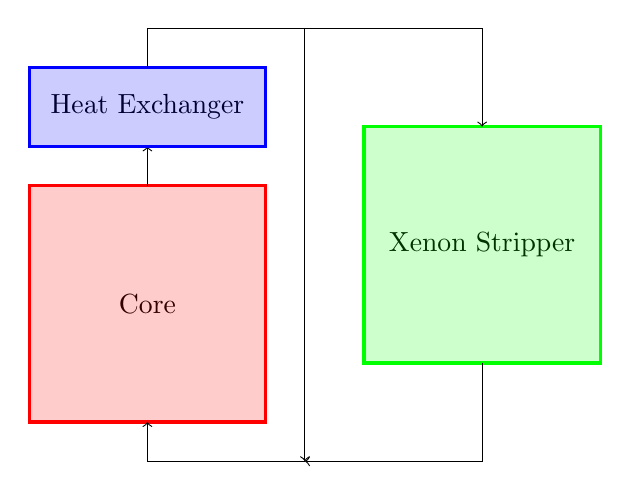
\begin{tikzpicture}
    %Core
    \draw node at (1.5,1.5) {Core};
    \draw[red, very thick] (0,0) rectangle (3,3);
    \filldraw[red,opacity=0.2] (0,0) rectangle (3,3) ;
    %Short Line
    \draw[->] (1.5,3) -- (1.5,3.5);
    %HEX
    \draw node at (1.5,4) {Heat Exchanger};
    \draw[blue, very thick] (0,3.5) rectangle (3,4.5);
    \filldraw[blue,opacity=0.2] (0,3.5) rectangle (3,4.5) ;
    %Inner Line
    \draw[->] (1.5,4.5) -- (1.5,5) -- (3.5,5)  -- (3.5,-0.5);
    \draw[->] (3.5,-0.5)  -- (1.5,-0.5) -- (1.5,0);
    %Stripper
    \draw node at (5.75,2.25) {Xenon Stripper};
    \draw[green, very thick] (4.25,3.75) rectangle (7.25,0.75);
    \filldraw[green,opacity=0.2] (4.25,3.75) rectangle (7.25,0.75) ;
    %Outer line
    \draw[->] (3.5,5)  -- (5.75,5)  -- (5.75,3.75);
    \draw[->] (5.75,0.75) -- (5.75,-0.5) -- (3.5,-0.5) ;
\end{tikzpicture}

    \caption[Block Flow Diagram - Molten Salt Microreactor with Xenon Stripping Module]{Block Flow Diagram - Molten Salt Microreactor with Xenon Stripping Module. The fuel/coolant salt mixture is heated by fission in the core, rises to the heat exchanger where it gives up heat to the secondary coolant and sinks by natural circulation. }
    \label{fig:BFD}
\end{figure}

\acf{oak} has studied a method of stripping xenon out of molten salt fuels during operation \cite{ORNL-masstransport}, in a way depicted by \cref{fig:BFD}. Helium bubbles are injected into the liquid fuel outside of the core and flow with the fuel before the phases are separated and a poison-poor stream returns to the core. This was primarily focused on the kinetics of a sparge tube stripper, and proposed an experiment to determine the mass transfer coefficients of dissolved xenon gas into fine helium bubbles. Such data is instrumental in the design of a mass transport unit operation, but unfortunately records of the experiment being conducted cannot be found. We seek to determine whether a return to the proposed experiment would be productive by conducting a thermodynamic analysis on the equilibrium system. More detailed design of such a stripper would be warranted if the thermodynamic analysis yields promising results.

It is worth noting the difference between the stripping operation described in this paper and off-gas management systems that all \acsp{msr} require \cite{Offgas}. Off-gas systems remove fission gases that naturally make their way into the head-spaces of the primary coolant loop of an \acs{msr}. Other work has concluded that a large fraction of fission gasses, including \Xe, fail to transport to the head-space, remaining dissolved due to poor liquid-gas interface, entrained due to the lack of nucleation sites, or flowing in circulating voids due to surface tension \cite{XeMSR}. Stripping greatly improves the kinetics of fission gas removal, and is more akin to fuel reprocessing, while the off-gas management system is more akin to the cladding gap in solid fuel designs.

While the present work is centered around removing gaseous poisons from \acs{msr} fuel, previous researchers have expressed interest in doing the opposite, and dissolving gaseous poisons such as boron-trifluoride into the melt for reactivity control \cite{BF3}. The transport delay of such actuation is likely to be on the order of seconds/minutes, while the effective neutron lifetime, which characterizes the neutron chain reaction, is on the order of tens/hundreds of milliseconds \cite[Ch. 1]{DH}. As such, soluble boron is not a suitable means of actuation for set-point tracking and is best reserved for fuel-reactivity shimming over the life of the reactor. Similarly, \Xe stripping is not practical for operational control and is only being studied for its open loop effects.

\section{Xenon-135 Decay Chain}\label{sec-decay}
One of the goals of this paper is to model xenon poison transients in \acsp{msr}. Therefore, it is important to understand the physics of the decay chain, particularly during dynamic time periods such as start-up, power transients, shut-down, and restart. The concentration of xenon-135 at a given time is described by a system of first-order \acfp{ode} which quantify the generation, consumption, and decay of itself and iodine-135:

\begin{equation}\label{eq:diffI}
    \frac{dI}{dt} =
    \underbrace{\gamma_{I}\Sigma_{f}^{F}{\phi}(t)}_{\text{Fission Yield}}
    -\underbrace{\lambda_{I}I(t)}_{\text{Beta Decay}}
\end{equation}
\begin{equation}\label{eq:diffXe}
        \frac{dXe}{dt} =
        \underbrace{\gamma_{Xe}\Sigma_{f}^{F}{\phi}(t)}_{\text{Fission Yield}}
        +
        \underbrace{\lambda_{I}I(t)}_{\text{Precursor Decay}}
        -\underbrace{\lambda_{Xe}Xe(t)}_{\text{Beta Decay}}
        -\underbrace{Xe(t)\sigma_{a}^{Xe}{\phi}(t)}_{\text{Radiative Capture}}
\end{equation}

\ref{eq:diffI} and \ref{eq:diffXe} can be used to track the concentrations of \I and \Xe during steady-state or dynamic operation \cite[Ch. 7]{Lamarsh}. Each nuclide is formed by \U[235] fission, and removed by beta-decay. Additionally, \Xe is formed by the beta-decay of \I and removed by radiative neutron capture. In reality, the decay chain is a bit more complicated than this. $^{135}Te$, the direct beta-precursor to \I is also formed by \U[235] fission \cite{Roberson}. Its half-life is orders of magnitude shorter than \I, so it is common to neglect its formation and instead lump its fission yield with \I. \Xe[135m] is also formed by \I beta-decay and is neglected for similar reasons. Neutron flux ($\phi$) exists on an energy spectrum, which effects the fuel-fission cross-section ($\Sigma_{f}^{F}$) and the \Xe poison cross-section $\sigma_{a}^{Xe}$. The form of \ref{eq:diffI} and \ref{eq:diffXe} in this work uses 1-group cross-sections and fluxes, which requires the use of neutron energy-integration, which is usually performed using a weighted-finite sum methodology. 

\subsection{Equilibrium Poisoning}
Following start-up, the nuclides builds-up in the reactor until the formation terms (i.e. fission yield and precursor decay) equilibrate with the removal terms (beta decay and radiative capture). By setting the time derivatives to zero in \ref{eq:diffI} and \ref{eq:diffXe}, the neutron flux dependent equilibrium concentrations may be derived algebraically \cite[Ch. 7]{Lamarsh}:

\begin{equation}\label{eq:I_eq}
    I_{\infty}(\phi) = \frac{\gamma_I \Sigma_f^F }{\lambda_I}\phi
\end{equation}
\begin{equation}\label{eq:Xe_eq}
    Xe_{\infty}(\phi) = \frac{(\gamma_I+\gamma_{Xe}) \Sigma_f^F }{\lambda_{Xe}+\sigma_a^{Xe}\phi}\phi
\end{equation}

When the power level (and therefore neutron flux) of the reactor is changed, the terms of \ref{eq:diffI} and \ref{eq:diffXe} are no longer balanced, and the nuclides move to a new equilibrium level along a path defined by the system of \acsp{ode}. The equilibrium \Xe can be converted to poison reactivity  by writing the one-group neutron balance equation for the explicit contribution of neutron capture by \Xe and assuming that the reactor is critical in the absence of \Xe. This is essentially the fraction of fission neutrons in a given generation that are captured by \Xe \cite{Bateman}.

\begin{equation}\label{eq:Xe_poison}
    \rho_{Xe}=-\frac{\sigma_a^{Xe}Xe_\infty}{\nu\Sigma_f^F}  
\end{equation}

\subsection{Reactor Shutdown}
\begin{table}[ht!]
    \caption[Relevant nuclear constants]{Relevant nuclear constants \cite{Lamarsh}. The \I fission yield ($\gamma$) is the sum of direct and indirect fission. The \I microscopic neutron capture cross-section ($\sigma$) is neglected as it is so small that it is insignificant compared to its own decay rate and the \Xe cross-section.}
    \centering\begin{tabular}{c|ccc}
                   &  $\gamma \;(\%)$ &  $\lambda \; (hr^{-1})$ &  $\sigma_a \; (Mb)$ \\ \hline
        \I  & 6.39            & 0.1035                 & -                \\
        \Xe & 0.237           & 0.0753                 & 2.65\textsuperscript{*}
    \end{tabular}\\
    \textsuperscript{*}At 0.025 eV
    \label{tab:params}
\end{table}
When the reactor is scrammed, each flux-containing term in the system of \acsp{ode} goes to zero, and the concentrations of the two nuclides are described by the Bateman equations \cite{Bateman}, which have a readily available solution given some initial condition \cite[Ch. 1]{Lamarsh}:

\begin{equation}\label{eq:I_bateman}
    I(t) = I_{\infty}e^{-\lambda_I t}
\end{equation}
\begin{equation}\label{eq:Xe_bateman}
    Xe(t) = Xe_{\infty}e^{-\lambda_{Xe} t}+I_{\infty}\frac{\lambda_I}{\lambda_I - \lambda_{Xe}}(e^{-\lambda_{Xe}t}-e^{-\lambda_{I}t})
\end{equation}

In this case the initial conditions are the equilibrium levels described by \ref{eq:I_eq} and \ref{eq:Xe_eq}. \I follows simple exponential decay. \Xe has a longer half-life than \I, as well as a lower equilibrium concentration (owing to its huge radiative capture cross-section). This results in an inverse response, where the \Xe concentration initially spikes before its decay rate exceeds its formation. \Cref{tab:params} contains literature values for the constants relevant to the iodine-xenon system. The time between the scram and the peak \Xe concentration, can be calculated by setting the derivative of \ref{eq:Xe_bateman} to zero:

\begin{equation}\label{eq:Xe_peak}
    t_{max} = \frac{ln\left(\frac{\lambda_{Xe}}{\lambda_{I}^2}\frac{Xe_{\infty}}{I_{\infty}}\right)\left(\lambda_{I}-\lambda_{Xe}\right)+\frac{\lambda_{Xe}}{\lambda_{I}}}{\lambda_{Xe}-\lambda_{I}}
\end{equation}

\ref{eq:Xe_peak} demonstrates that the time of the xenon peak depends mostly on the decay constants of \Xe and \I, with only a weak dependence (logarithmic and buffered) on $\nicefrac{Xe_{\infty}}{I_\infty}$. By inspection of \ref{eq:I_eq} and \ref{eq:Xe_eq}, it can be observed that this equilibrium nuclide ratio is only weakly dependent on the power level of the reactor before the scram. $\Sigma_f\phi$ cancels out, leaving the contribution of neutron capture to the effective half-life\footnote{\label{fn:EHL} Effective half-life quantifies the actual removal rate of a species by aggregating all removal modes, in this case beta-decay and neutron capture. For transmutation,} $\sigma_a^{Xe}\phi$ is analogous to the decay constant \cite[Ch. 7]{Lamarsh}.
of \Xe as the only flux containing term that impacts $t_{max}$ 


\subsection{Reactor Restart}
When the fission chain reaction is restarted, the neutron flux increases and resumes transmuting \Xe. This shortens the effective half-life\footref{fn:EHL} of the poison, accelerating the removal rate which is already high, owing to the elevated concentration. The removal of poisons is akin to positive reactivity insertion \cite{Roberson}. Decreasing poison concentration increases the neutron population and therefore the rate of poison removal. This is a positive feedback system which could escalate and disturb the temperature of downstream systems such as power cycles and process heat applications if control reactivity is not removed to match. As such, regulation and standard operating procedures may restrict or ban the restart of a reactor in a super-equilibrium state, and operators typically must wait until the \Xe level returns to near the full-power equilibrium level to restart \cite{CFR}.

The duration of the xenon dead-time could be shortened by adding an additional negative term to \ref{eq:diffXe}. This is not physically realizable in our current fleet of cladded solid fuel reactors. Vented solid nuclear fuel elements have been conceptualized for high temperature reactors which have high partial pressure from fission products \cite{VentPatent,VentedRods}. Still, this concept only allows for the venting of fission gasses due to positive pressure within the fuel element. Even if a flowing sweep gas were incorporated to further facilitate fission gas removal, a vented rod's ability to manipulate neutron poison concentration within the fuel will be limited by the diffusion of xenon through the fuel matrix \cite{XeDiffuse}.

It is however possible to strip a gaseous solvent from a liquid such as \acs{msr} fuel. Xenon, being a noble gas, is weakly dissolved in the molten salt, and it is more energetically favorable for it to exist as a gas. A gas bubble cannot form spontaneously and requires a nucleation site to surmount the associated activation energy barrier \cite{reviewXeMSR}. This often comes in the form of an impurity that has a trapped bubble attached. When a xenon atom comes into contact with the salt/gas interface, it transports into the bubble. When the bubble grows large enough, it will stop circulating and get caught in the reactor head-space where the off-gas system can remove it. 

Instead of waiting for such a chance incident to occur, a bulk gas phase can be bubbled through the salt, which provides interfacial area across which and volume into which the xenon will preferentially transport through an operation called stripping \cite[Ch. 10]{Geankoplis}. \cite{ORIGEN} has studied the off-gassing of nobel gas fission products from liquid fueled \acs{msr}, including the \acs{msre}. This was modeled using flow blocks in SCALE's TRITON sequence by assuming or calculating a removal constant for fission gasses that transport into the off-gas. The present work extends upon this idea by deriving a removal constant composed from optionally time dependent parameters for a single stage equilibrium stripper, and implementing it in an open source solver. For this purpose \ref{eq:diffXe} is modified with the addition of the stripping term which will be derived in Section \ref{sec-masstransport} (\ref{eq:diffXe_strip_generic}).

\section{Methodology}\label{sec-meth}
A two pronged methodology is employed to model the xenon-iodine decay chain in an \acs{msr} with the addition of xenon stripping. A unique model was derived to describe the thermodynamic equilibrium products of a unit operation that removes dissolved and entrained xenon gas from a molten salt by preferential transport into a bulk helium stream (see Section \ref{sec-masstransport}). This model is combined with the well understood model of the \Xe system described in Section \ref{sec-decay} to form \ref{eq:diffXe_strip}, which is the basis for this work and is solved numerically in Section \ref{sec-script}. 

\begin{equation} \label{eq:diffXe_strip_generic}
    \frac{dXe}{dt} =
        \underbrace{\gamma_{Xe}\Sigma_{f}^{F}{\phi}(t)}_{\text{Fission Yield}}\;+\underbrace{\lambda_{I}I(t)}_{\text{Precursor Decay}}
        -\;\underbrace{\lambda_{Xe}Xe(t)}_{\text{Beta Decay}}
        \;-\;\underbrace{Xe(t)\sigma_{a}^{Xe}{\phi}(t)}_{\text{Radiative Capture}}
        \;-\left(\frac{dXe}{dt}\right)_{strip}
\end{equation}

\subsection{Two-phase Equilibrium Mass Transport}\label{sec-masstransport}
The stripping term from \ref{eq:diffXe_strip_generic} is derived in this section. Dissolved gasses follow Henry's law, at low concentration: 

\begin{equation}\label{eq:henry}
    C_{\ell} = Hp
\end{equation}

 This describes a relationship between the concentration of the solute in the liquid phase ($C_{\ell}$) and the partial pressure of the solute in the cover gas ($p$) when the two phases are in equilibrium \cite[Ch. 10]{Geankoplis}. Fresh cover gas can be supplied to strip the solute into the cover gas. By considering total pressure of the cover gas and assuming an equation of state, Henry's law can be modified to be expressed in terms of gas phase concentration instead of partial pressure, as shown by: 

\begin{equation}\label{eq:henry-modified}
    C_{\ell} = H^{*}C_g
\end{equation}

An early study conducted at \acs{oak} predicted such a unitless Henry's Law constant ($H^*$) for the xenon-FLiNaK system on the order of $1 \times 10^{-4}$ at MSR temperatures \cite{ORNL-solubility}. While \cite{ORNL-solubility} did not experimentally validate this specific prediction, it did show through experimentation with lighter noble gasses that the formula used to make the prediction was accurate at the order of magnitude level. This level of precision should be refined in future work but is acceptable for this high-level analysis. The solver is and will continue to be open source, allowing future researchers to refine  parameters such as $H^*$, including writing a simple plug-in to allow for potential time-variability in $H^*$ due to burn-up and temperature.

Consider a co-current sparge pipe stripper that uses fresh helium to remove dissolved and entrained xenon from molten salt fuel. The helium does not react and simply provides a bulk gas phase for macroscopic-scale xenon transport. If the interfacial area in the pipe is sufficient, the xenon concentration in the outlet-gas stream will be in equilibrium with that of the liquid outlet. \cref{fig:strip} is a schematic drawing of such a stripper and shows the xenon concentration at the inlet and outlet of the molten salt and gas streams, as well as the volumetric flow rate of each stream. 

\begin{figure}[ht!]\centering
    \resizebox*{0.75\textwidth}{!}{\begin{tikzpicture}
    \draw[green, very thick] (-2,-0.5) rectangle (2,0.5) ;
    \filldraw[green!10] (-2,-0.5) rectangle (2,0.5);
    \draw node at (0,0) {\small Xenon Stripper};
    %Bottom
    \draw[->,blue] (-1.5,-2)--(-1.5,-0.5);
    \draw node at (-1.35,-1.55) [anchor=west]{\small{$C_{He}^{in} = 0$}};
    \draw node at (-1.65,-1.55) [anchor=east]{\small{$\dot{V}_{He}$}};
    %Top
    \draw[->,blue] (1.5,0.5)--(1.5,2);
    \draw node at (1.65,1.55) [anchor=west]{\small{$C_{He}^{out} = \nicefrac{C_{salt}^{out}}{H^*}$}};
    \draw node at (1.35,1.55) [anchor=east]{\small{$\dot{V}_{He}$}};
    %Left
    \draw[->,red] (-3.75,0)--(-2,0);
    \draw node at (-2.0,0.5) [anchor=east]{\small{$C_{salt}^{in} = Xe(t)$}} ;
    \draw node at (-3.0,-0.5) {\small{$\dot{V}_{salt}$}} ;
    %Right
    \draw[->,red] (2,0)--(5,0);
    \draw node at (2.0,0.5) [anchor = west]{\small{$C_{salt}^{out} = C_{salt}^{in}-C_{He}^{out}\frac{\dot{V}_{He}}{\dot{V}_{salt}}$}};
    \draw node at (3.0,-0.5) [anchor=west]{\small{$\dot{V}_{salt}$}} ;
    \end{tikzpicture}
    
}
     \caption[Schematic Drawing of Xenon Stripping Module]{Schematic Drawing of Xenon Stripping Module. Fresh helium and molten salt with a given} \Xe concentration enters on the left. Dissolved and entrained xenon preferentially transports from the liquid phase to the gaseous stream. Loaded helium and molten salt with a lower \Xe concentration exit on the right. The exiting streams are in equilibrium with each other according to Henry's Law. 
    \label{fig:strip}
\end{figure}
\note{why is the caption centered}
The salt enters with \Xe concentration equal to that of the xenon level in the core, and exits at some lower value. The helium enters with no xenon, and exits with a \Xe concentration in equilibrium with the salt's outlet concentration. This analysis is based on the horizontal co-current sparge pipe designed at \acs{oak} during the \acf{msre} \cite{ORNL-masstransport}. A counter-current design may allow for greater stripping effectiveness by maintaining a more constant (and therefore a larger log-mean average) driving force, but it makes the separation of phases more challenging. The horizontal design also eliminates hydrostatic pressure differential across the unit operation, so a constant volumetric gas-phase flow rate constant across the module can be assumed.


A simple mass balance shows that the concentration in the liquid outlet must be equal to the inlet concentration minus the gas outlet concentration times the gas-to-liquid volumetric flow rate ratio. As shown in \cref{fig:strip}, substituting the definition of $C^{out}_{He}$ into the definition of $C^{out}_salt$, we obtain:

\begin{equation} \label{eq:saltout}
    C_{salt}^{out}=C_{salt}^{in}\left( 1+\frac{1}{H^*}\frac{\dot{V}_{He}}{\dot{V}_{salt}}  \right)^{-1}
\end{equation}

The local (e.g. inside of the xenon stripping module) change in xenon-135 concentration can be simplified by substituting the definitions of $C_{He}^{out}$ and $C_{salt}^{out}$ from \cref{fig:strip} into \ref{eq:saltout}:  


\begin{equation} \label{eq:local_diff}
    dC_{salt} = {C_{salt}^{in}}\left( H^*\frac{\dot{V}_{salt}}{\dot{V}_{He}}+1 \right)^{-1}
\end{equation}

Over a certain amount of time ($dt$), only some fraction (determined by the \acs{msr} flow period) of the molten salt will pass through the xenon stripping module.  Therefore, $\left(\nicefrac{dXe}{dt}\right)_{strip}$ appearing in \ref{eq:diffXe_strip_generic} is given by : 

\begin{equation}\label{eq:dXedt-strip}
    \left(\frac{dXe}{dt}\right)_{strip} = \tau_{salt}^{-1}{dC_{salt}}
\end{equation}



\ref{eq:diffXe_strip_generic} can then be re-written as 
below, where the inverse of $\tau_{salt}(H^*\nicefrac{\dot{V}_{salt}}{\dot{V}_{He}}+1)$ is analogous to the decay constant for stripping: 
\vspace{-0.5\baselineskip}
\begin{equation}\label{eq:diffXe_strip}
        \frac{dXe}{dt} =
        \underbrace{\gamma_{Xe}\Sigma_{f}^{F}{\phi}(t)}_{\text{Fission Yield}}
        +\underbrace{\lambda_{I}I(t)}_{\text{Precursor Decay}}
        -\underbrace{\lambda_{Xe}Xe(t)}_{\text{Beta Decay}}
        -\underbrace{Xe(t)\sigma_{a}^{Xe}{\phi}(t)}_{\text{Radiative Capture}}
        -\underbrace{ \frac{Xe(t)}{\tau_{salt}}\left( H^*\frac{\dot{V}_{salt}}{\dot{V}_{He}}+1 \right)^{-1}}_{\text{Stripping}}
\end{equation}

This derivation neglects the positional variance of xenon-135 concentration resulting from the stripper. This simplification is reasonable when the salt traverses the flow loop multiple times while the xenon stripping module is active; i.e, the flow period is small compared to the restart time.

The stripping term in \ref{eq:diffXe_strip} is mathematically undefined at zero helium flow rate. It can logically be inferred (and shown by taking the limit of the term as $\dot{V}_{He}$ approaches zero) that such a case corresponds to zero stripping change.

\subsection{Numerical Solver} \label{sec-script}
A numerical solver was derived in Python 3.10 to track the time dependent \I and \Xe concentrations while giving the user control over the neutron flux and helium flow rate throughout the process\footnote{The numerical solver is available at \href{https://github.com/sjroot97/NumericalSolverXe135}{https://github.com/sjroot97/NumericalSolverXe135}. The version of the solver used to plot \cref{fig:PeakRestart} is included in Appendix \ref{app:solver} as an example. Users are permitted free use of the solver with the condition that any refinements, advancements, or plug-ins built-on also be shared freely.} This allows the user to investigate the change in xenon poisoning after a power change, and the effectiveness of the equilibrium stripper characterized in Section \ref{sec-masstransport} in shortening the post-scram restart time in an \acs{msr}. Euler's forward method is applied, where the nuclide concentrations for the next time step are calculated 
using the current concentrations and the current rates of change, given by \ref{eq:diffI} and \ref{eq:diffXe_strip}:

\begin{equation}\label{eq:I_Euler}
    I[t+dt]=I[t]+\frac{dI}{dt}[t]
\end{equation}
\begin{equation}\label{eq:Xe_Euler}
    Xe[t+dt]=Xe[t]+\frac{dXe}{dt}[t]
\end{equation}

The solver is object oriented, which makes it modular and allows code to be re-used for both \I and \Xe. The class `Core' contains constants such as the macroscopic fission cross-section ($\Sigma_f^F$) and key variables, most notably the neutron flux and helium flow rate. It also contains class methods that can be used to modify each of the aforementioned variables to simulate a scram and activation of the xenon stripping module. The class `Nuclide' serves as the framework for the simulation. An object containing all physical constants and parent-daughter relationships is instantiated for \I and \Xe. It also contains methods to calculate each term of \ref{eq:diffI} and \ref{eq:diffXe_strip} which are combined to track the concentrations using \ref{eq:I_Euler} and \ref{eq:Xe_Euler}.


A time step length ($dt$) of 1 second was selected to strike a balance between precision and computational intensity. The solver is able to simulate hundreds of hours of nuclide evolution in under a minute on an HP laptop with a 2.3 GHz Intel Core i7 processor and 12 GB of memory, without long time-steps (e.g. on the order of the nuclide's half-life) which would cause  local truncation error. This is long enough to allow the \Xe concentration to equilibrate, and an entire dynamic case study to be conducted.

To conduct a case study, the solver iterates over a time loop, appending the new concentration of \I and \Xe at each time step.  At any time, the prompt neutron flux and helium flow rate may be independently changed by using class method `scram' and `strip'. These two methods are used in conjunction to conduct the experiments discussed in Section \ref{sec-res}.

Class method `scram' can optionally call a subroutine (class method delayed\_neutron\_precursors) that creates a list of delayed neutron flux following shutdown ($\phi^{d}(t)$) using the six-group approximation and the data in \Cref{tab:precursors}, obtained from \cite{Kerlin}:

\begin{equation}\label{eq:dn_flux}
    \phi^{d}(t) = \phi_{0} \vec{\beta} \cdot e^{-t\vec{\lambda}}
\end{equation}

The solver then checks if the list contains values, and removes the zeroth value, assigning it to be the new flux using the `pop' method. This approach can be used to treat any parameter assumed to be constant in this paper as a time-variable.

\begin{table}[ht!]
    \caption[Delayed neutron data]{Delayed neutron fraction ($\beta$) and decay constant ($\lambda$) for \U[235] \cite{Kerlin}. The total delayed neutron fraction is 0.67\%}
    \centering\begin{tabular}{c|cc}
    Group  & $\beta \;(\%)$   & $\lambda \; (s^{-1})$ \\ \hline
        1  & 0.0221           & 0.0124 \\ 
        2  & 0.1467           & 0.0305 \\
        3  & 0.1313           & 0.111  \\ 
        4  & 0.2647           & 0.301  \\ 
        5  & 0.0771           & 1.14   \\ 
        6  & 0.0281           & 3.01   \\               
    \end{tabular}\\
    \label{tab:precursors}
\end{table}


\section{Results and Discussion} \label{sec-res}

\subsection{Input Data}
A \acs{msnb} concept was used as a case study. This design uses 19.75\% enriched $UF_4$ derived from \acf{haleu} as a fuel salt, and dissolved at 18 mol\% in FLiNaK, a eutectic mixture of three alkaline fluoride salts: LiF, NaF, and KF \cite{CarterNumerical}. This is an epithermal (0.167 eV) reactor with microscopic fission cross-section of $\sigma_{f}^{235}\approx 180\; b$ and a microscopic \Xe neutron absorption cross-section of $\sigma_{a}^{Xe}\approx 430\; kb$ \cite{TENDL}. The core is a $166\; cm$ tall right cylinder $25\; cm$ in radius, and has a nominal transport time of $\tau_{salt} \approx 130\; s$. With a primary coolant loop length (which has equivalent cross-section) of $571\; cm$, this corresponds to a volumetric flow rate of $8.26 \; L/s$. The reactor is operated at low flux in the interest of fuel longevity \cite{CarterNumerical}.  At a more typical core average epithermal neutron flux of $10^{14} \; n/cm^{2}-s$, the reactor would generate around 200 MWth of power, approaching the power density limit of liquid fueled molten salt reactors \cite{PowerDensity}. 

The generic \acs{msr} reactor has been designed with constant flow-cross section, meaning that half of the salt is inside the core and half is outside. The overall volume-integrated average flux is therefore $5\times 10^{13} n/cm^3-s$ to account for the time the salt spends in the downcomer. As this is a natural circulation design, the higher power would result in a higher mass flow rate, but for the purposes of this study, it is assumed that a reactor designed to operate at this higher flux will include additional valving to add sufficient pressure drop to hold the nominal transport time at $\tau_{salt} \approx 130\; s$.

Natural circulation systems in the fully developed turbulent flow regime have a cubic relationship between the mass flow rate and the thermal power transported\cite[Ch. 3]{TodreasKazimi2}. In the hours after shutdown, decay heat accounts for 3-5\% of full power \cite[Ch. 3]{TodreasKazimi1}, so the hot-standby flow rate should drop to about 30-35\% of the operational flow rate. As such, the class method `scram(cls)' also increases $\tau_{salt}$ by a factor of 3 which represents managing decay heat in a roughly isothermal manner.



\subsection{Case Studies}
\subsubsection{Benchmark Study}

First, a base case study was conducted where the xenon stripping module remained off for the entire experiment. The reactor is started, operates until \I and \Xe levels equilibrate, and is scrammed. The results given by the numerical solver are compared with characteristic stationary points of the analytical solutions so that the model can be benchmarked before moving on to studies where the stripping term is required.

The \Xe and \I concentration profiles during a clean start-up are depicted by \cref{fig:startup}. The \I level rises to an equilibrium concentration of 28.4 $\nicefrac{mmol}{m^3}$ as a first order response over the course of two days. The \Xe level follows an over-damped second order response to the its equilibrium level (denoted by the horizontal dashed line) of 20.0 $\nicefrac{mmol}{m^3}$. Using \ref{eq:Xe_poison}, equilibrium xenon accounts for -1.38\% of poison reactivity. The `shoulder' during the first few hours is formed because its primary source, precursor decay, is initially null. Similarly, the elongation of the curve is caused by the changing formation rate as the \I concentration rises. 

\begin{figure}[ht!]
    \centering
    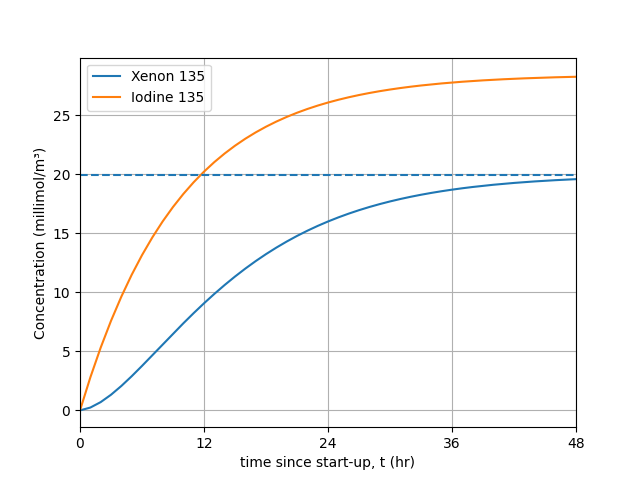
\includegraphics[width=0.75\textwidth]{Xenon/start-up}
    \caption[Concentration of \I and \Xe vs. time following start-up]{Concentration of \I and \Xe vs. time following cold/clean start-up. \I and \Xe are formed by fission as soon as the reactor starts. Soon after, \I decays to \Xe, and \Xe captures neutrons, being transmuted to \Xe[136]. These two species reach equilibrium values when generation and consumption are equal.}
    \label{fig:startup}
\end{figure}

After \I and \Xe equilibrate, the reactor is scrammed by setting the prompt neutron flux to zero, subsequently producing the behavior shown in  \cref{fig:Control}. The \I concentration falls by simple exponential decay, while the \Xe concentration undergoes a second order response with numerator dynamics, peaking at 23.11 $\nicefrac{mmol}{m^3}$ 7 hours after the scram. The -1.60\% xenon reactivity at the peak represents a 16\% super-equilibrium. The \Xe concentration crosses its full power equilibrium 12.4 hours after the scram, which is denoted by a vertical dashed line. Delayed neutrons make a small contribution over the hours following shutdown, decaying from 0.67\% to 1 ppm of the full power flux in under 8 minutes. Impact to the \Xe concentration profile was estimated to be at the part-per-billion order by inspection of results with and without the delayed neutron subroutine.

\subsubsection{Verification of the Numerical Solver} 
For the given inputs, \ref{eq:I_eq} and \ref{eq:Xe_eq} predict an equilibrium \I concentration of 28.4 $\nicefrac{mmol}{m^3}$, and an equilibrium \Xe concentration of 19.96 $\nicefrac{mmol}{m^3}$. \ref{eq:Xe_peak} predicts that the peak of the inverse response occurs 5.1 hours and 3 minutes after the reactor is scrammed, with a magnitude of 23.1 $\nicefrac{mmol}{m^3}$ obtained by inserting the peak time into \ref{eq:Xe_bateman}. The analytic solutions of characteristic stationary points of the system of \acsp{ode} give identical results with respect to the numerical solver, verifying the results of the model for the benchmark study. 

To further verify the numerical solver, the path by which nuclide concentration approaches equilibrium can be compared to analytical solutions. By making the simplification of constant (time-independent) neutron flux, an analytical solution can be obtained for the \I concentration:

\begin{equation}\label{eq:I_analytical}
\left.I(t)\right\rvert_\phi = (I_o-I_\infty)e^{-\lambda_I t}+I_\infty
\end{equation}

The accuracy of the numerical solver was quantified by comparing the \I concentration array to \ref{eq:I_analytical}. An $1-r^2$ score of $1.46\times10^{-8}$ was obtained over the first 48 hours of start-up. This value is not sensitive to the initial condition, with approximately the same $r^2$ value being observed regardless of the \I level at start-up. This was tested over a range from 10\% to 5 times the equilibrium value.

\begin{figure}[ht!]
    \centering
    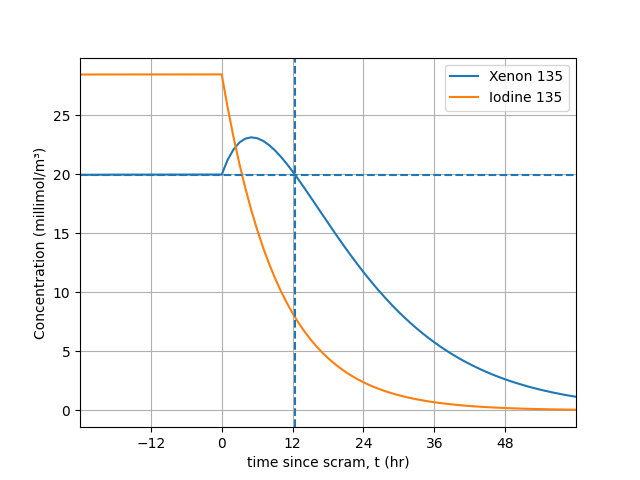
\includegraphics[width=0.75\textwidth]{Xenon/noHe}
    \caption[Concentration of \I and \Xe vs. time following reactor scram]{Concentration of \I and \Xe vs. time following reactor scram. When the reactor is scrammed, fission and transmutation cease. \I and \Xe each continue decaying. Initially, \I decays at a higher rate due to the shorter half-life and larger population. The \Xe concentration reaches its peak when the rate of \I decay drops below the rate of \Xe decay. After the equilibrium value is passed, the reactor may be restarted safely.}
    \label{fig:Control}
\end{figure}

The \Xe rise to equilibrium is more difficult to analytically solve, owing to the variable generation rate caused by the changing decay rate of \I. Because $I_\infty$ is already known, we can choose this as $I_o$, which makes the \I concentration and \Xe generation rate constant at $\gamma_{Xe}\Sigma_{f}^{F}{\phi}$ and the ODE separable. This is not a physically meaningful calculation, but it does hold mathematical meaning, and the solver is capable of computing it. The solution to this simplified ODE has the same form as \ref{eq:I_analytical}, with the effective decay constant, $\lambda_{Xe}+\sigma_a^{Xe}\phi$, in the exponent. By replicating the assumptions of the simplified ODE, the numerical solver was found to have an $r^2$ value of essentially 1. During normal operation of the solver, some error propagation is expected which would cause the numerical \Xe solution to be slightly less precise. However the low error calculated in the \I verification limits the effect of error propagation.

The \I verification gives assurance that the fission yield and beta decay methods work as intended, while the \Xe scenario verifies the radiative capture method. To verify the precursor decay method, \ref{eq:I_bateman} and \ref{eq:Xe_bateman} are compared to the numerical solutions, obtaining $1-r^2$ scores of $1.05\times10^{-9}$ and $4.59\times10^{-10}$. The level of precision achieved by the numerical solver in the verification studies gives confidence that it will accurately predict the behavior in more complicated studies, for which analytical solutions are difficult to obtain.

\subsubsection{Super-Equilibrium Restart}
The first experiment was repeated, but this time the reactor was restarted at the xenon peak, producing the behavior shown in \cref{fig:PeakRestart}. 96 pcm of \Xe burned out in the first hour, and the \Xe reactivity dipped to 120 pcm below its equilibrium level 10.4 hours after the reactor was restarted. 

\begin{figure}[ht!]
    \centering
    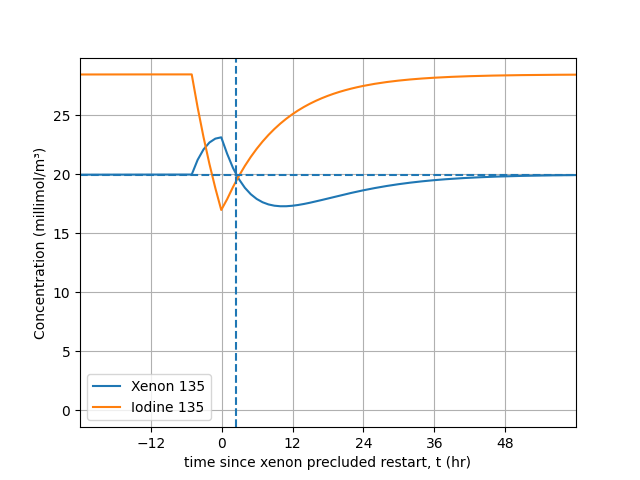
\includegraphics[width=0.75\textwidth]{Xenon/peakrestart}
    \caption[Concentration of \I and \Xe vs. time following restart at xenon peak]{Concentration of \I and \Xe vs. time following restart at xenon peak. When the reactor is restarted, fission and transmutation resume. \I immediately builds back up, while \Xe burns out, returning to equilibrium after a substantial overshoot.}
    \label{fig:PeakRestart}
\end{figure}

This is a significant disturbance to the poison reactivity of the reactor during operation. The magnitude of the reactivity swing during the restart is equivalent to 25\% of the difference between clean start-up and equilibrium xenon poisoning, and the maximum burnout rate is more than 1.5 times the maximum \Xe build-up rate during initial start-up (63 pcm/hr). The most significant issue is that the burn-out of super-equilibrium \Xe during operation causes a positive feedback loop that the reactivity controller has to reject; if the drop in poison reactivity is not counteracted by control rod insertion, the neutron population grows, which increases the xenon burn-out rate.

With proper reactor and controller design, this disturbance can be managed. With a temperature coefficient of 3.5 pcm/K, the core temperature could swing by up to 27 degrees Celcius in the first hour, and 97 degrees overall \cite{CarterMCNP}. Depending on the hot standby temperature, coolant salt volatility limits could be approached. More likely, downstream systems such as power cycles and process heat applications may be disturbed, putting stress on the plant-wide distributed control system. While this may be manageable, it would be preferable, and potentially required, to avoid this type of re-start.

\subsubsection{Scheduled Restart}
An \acs{msr} deployed in a load-following capacity on an isolated grid may at times need to be shut down (or ramped down) overnight, then be powered up in the morning. The numerical solver was used to study such a scenario plotted in \cref{fig:Restart}. The \I concentration decays as in \cref{fig:Control}, and the \Xe concentration rises initially. Due to the stripping term in \ref{eq:diffXe_strip}, the peak is lower and occurs sooner, and the poison level crosses the equilibrium value sooner. The flow rate ratio ($\frac{\dot{V}_{He}}{\dot{V}_{salt}}$) required to return the \Xe concentration to its equilibrium value after 8 hours of dead-time is $2.15 \times 10^{-7}$. This corresponds to just 2.1 $\nicefrac{mL}{hr}$ of helium, or 16.8 mL over the entire dead-time. At approximately atmospheric pressure and 1000 K, this is such a small amount of helium that, if single-stage equilibrium is practically achievable, it may make more sense to release all of the necessary helium in a single pulse or series of pulses over the dead-time rather than continuously.

\begin{figure}[b!]
    \centering
    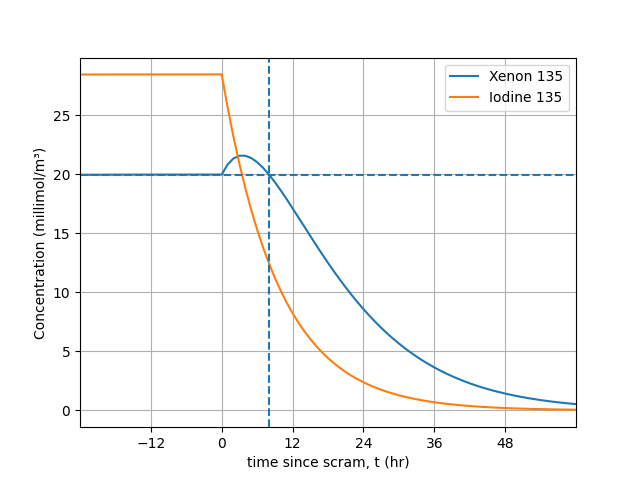
\includegraphics[width=0.75\textwidth]{Xenon/8hr_restart}
    \caption[Concentration of \I and \Xe vs. time following reactor scram - Restart Mode]{Concentration of \I and \Xe vs. time following reactor scram with Xenon Stripping Module. The same dynamics take place as in \cref{fig:Control}, except in this case the \Xe is also being removed from the molten salt fuel in the Xenon Stripping Module, so the reactor may be restarted in 8 hours.}
    \label{fig:Restart}
\end{figure}

Such a pattern may fit into the energy demands of a modest island population, for example Guam, where much less power is required overnight. Conventionally this would not be feasible as it would require powering up from hot-standby or low-power mode during the xenon peak. A xenon stripping module could be coupled to the reactor to shorten the super-equilibrium time period, and make it possible to produce electricity on schedule.

A more traditional method for accelerating the effective half-life below what is achieved by beta decay alone, is low power burn-out. Maintaining the shut-down reactor at 1\% power, which is on the order of the thermal power from decay heat, can reduce the effective half-life to 9.11 hours (compared to the half-life of 9.21 for pure beta decay). In comparison, the usage of the xenon stripper outlined in this experiment yields an effective half-life of 7.29 hours. This represents a 25 fold increase in the effectiveness of \Xe removal.

\subsubsection{Demand Response}
Power-peaking is another dynamic energy sector that must be decarbonized. An \acs{msnb} acting in this capacity will need to be able to black-start within minutes of a call for power. To return the \Xe concentration from its peak at 7.0 hours after shut-down to its equilibrium level in 390 seconds (3 hot-standby flow periods) requires a helium flow rate of 2.9 $\nicefrac{mL}{min}$, totalling 19 mL over the entire start-up procedure. \cref{fig:Standby} displays the \I and \Xe as calculated by the numerical solver with these settings. It is identical to \cref{fig:Control} until the peak poison level, when the xenon stripping module is activated and the \Xe level drops rapidly. 

If this standby restart was conducted every day for 10 years, it would require only 1 mole of helium gas. This is a conservative estimate due to the short duration that the xenon-stripping module is active. The solver instantly distributes the effect of the stripped xenon across the entire reactor. This prematurely depresses the mass transport driving force and therefore predicts a lower separation efficacy than would be observed in practice. Expansion of the solver to a 1D+time or multi-region lumped parameter model could improve the accuracy for this case study, at the expense of significantly more computational expense.

\begin{figure}[ht!]
    \centering
    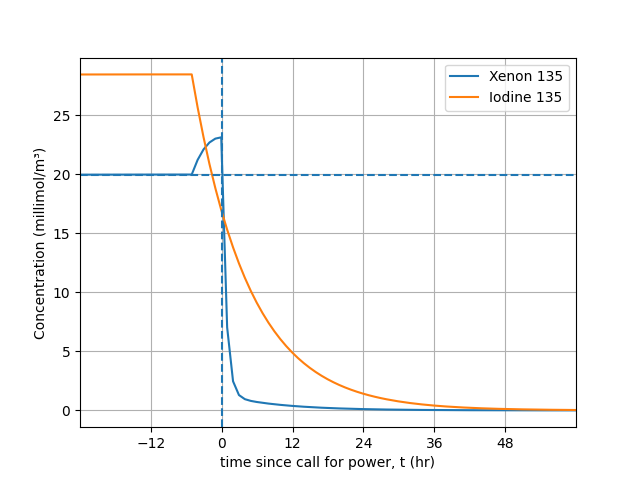
\includegraphics[width=0.75\textwidth]{Xenon/standby_restart}
    \caption[Concentration of \I and \Xe vs. time following reactor scram - Standby Mode]{Concentration of \I and \Xe vs. time following reactor scram with Xenon Stripping Module operating only immediately after the \Xe concentration reaches its peak. The same dynamics take place as in \cref{fig:Control}, except in this case \Xe is rapidly stripped from the molten salt fuel immediately after the \Xe concentration reaches its peak.}
    \label{fig:Standby}
\end{figure}

Operators of an \acs{msr} that is implemented in a power-peaking application will not know exactly when it needs to be restarted, but will need to have the reactor on standby. If this is the case, the xenon stripping module could remain off until the start-up signal comes. The module could then operate at a much higher helium flow rate than seen in the previous experiment for a short period of time similar to the start up time of our current natural gas peaking generators \cite{GE} before the \acs{msnb} is black-started. 

\subsubsection{End of Life Fuel}\label{sec-EOL}
 Molten salt microreactors such as the \acs{msnb} could extend their lifetime with xenon stripping. At the end of the fuel lifetime, excess reactivity could be reclaimed by constantly removing \Xe from the fuel, driving down the equilibrium concentration. A helium flow rate of 146 mL/hr reduces the equilibrium poison reactivity from 1.38\% to 0.15\%, a reduction of 1227 pcm. \cref{fig:EOLstartup} displays that the \I concentration is unchanged with respect to \cref{fig:startup}, while the \Xe concentration is greatly depressed. 
 
 Equilibrium xenon accounts for a significant amount of poison reactivity at high power density. Because microreactors are small, they are often limited in excess reactivity. They are also often designed to last upwards of a decade without refueling. For an \acs{msnb} with approximately 5\% excess reactivity at initial start-up, \Xe poisoning greatly reduces the fuel lifetime. A reduction in the equilibrium poison level such as the one described in this experiment requires 1270 L of helium per year, but could conceivably extend the overall reactor lifetime by up to 30\%.
This result alone, without considering the effect of shortening restart time, makes the xenon stripper an important design feature to small \acsp{msr}, which are competing for a market share in a class of reactors that are aiming for decade scale operation \cite{PetersonMS}.

\begin{figure}[ht!]
    \centering
    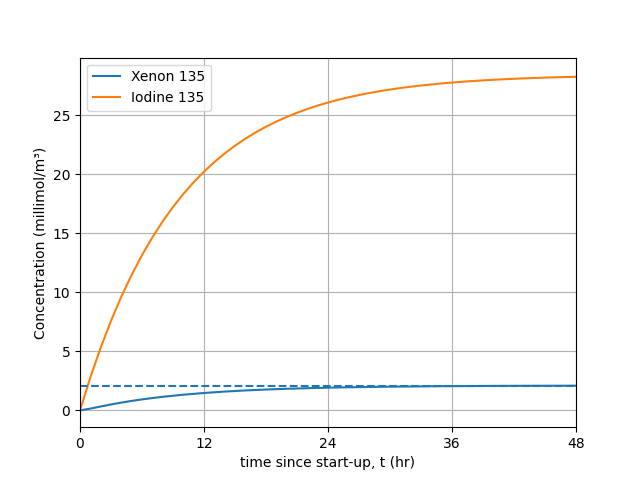
\includegraphics[width=0.75\textwidth]{Xenon/EOL-startup}
    \caption[Concentration of \I and \Xe vs. time during start-up - End of Life Fuel Mode]{Concentration of \I and \Xe vs. time during reactor start-up with Xenon Stripping Module operating to lower the equilibrium \Xe concentration.}
    \label{fig:EOLstartup}
\end{figure}


\section{Future work} \label{sec-fwk}
This work is a computational screening of xenon stripping for neutron poison management on a generic \acs{msr}, both during operation and during brief shut-down periods. Furthermore, it contains the development of a preliminary design tool that can be used to advise decisions in the specific design of \acsp{msr}. Many assumptions were made, notably a constant Henry's Law coefficient, which is subject to change during operation due to changing composition, and a constant natural circulation flow rate. These assumptions were made because of the lack of experimental data and the effect of design specifications on these parameters. By making the solver open source, we encourage other researchers to refine these assumptions as progress in experimental work supports.

\subsection{Xenon Stripping Module}
This paper works on the simplifying assumption that the xenon stripping module is an equilibrium mass transport unit operation. It has been demonstrated that the thermodynamics of \Xe stripping from molten salt fuel are highly favorable due to xenon's noble gas nature. This warrants a more detailed investigation into the kinetics of the unit operation. Literature must be consulted to design such a module \cite[Ch. 10]{Geankoplis}. It is highly likely that a higher helium flow rate will be required to prevent flooding and result in a sufficient interfacial area to volume ratio for mass transport to occur at any meaningful macroscopic rate. 

This paper also neglects the effect of other fission gasses that will be produced in the core, namely tritium. Core burn-up modeling will need to be conducted, and literature reviewed to see what other gasses may be stripped \cite{Offgas}. These additional gasses may inhibit xenon stripping by effecting the mass transfer coefficient, but will more likely facilitate improved stripping by contributing to the formation of circulating voids which may be removed from the salt more readily \cite{XeMSR}. 

\subsection{Numerical Solver}
The numerical solver is an object oriented program, making it modular. The architecture supports the instantiation of additional nuclides with a minimal amount of extra code. It could be used to study other equilibrium poison systems such as the \Sm decay chain, burnable poisons like gadolinium isotopes, and non-burnable poisons like hafnium isotopes. Outside of neutron poisoning, the solver could be modified to optimize isotope production schemes, track the gamma-ray source strength or decay heat potential of irradiated materials, or even estimate radiation damage and fission product interaction.

The solver is faster than real-time. A potential application beyond preliminary design is in control systems. A similar architecture could be employed to develop reduced-order just-in-time digital twins which would advise supervisory controllers during transient operations. This would allow, for example, the control system of a nuclear reactor to account for poison reactivity changes without having to wait for the disturbance to cause a set-point error, as would be required in a pure feedback controller.



\section{Conclusions} \label{sec-sum}
A new model was derived that quantifies the advective removal rate of \Xe from a molten salt fuel in an equilibrium stripper using Henry's law constants obtained from literature. It was used to demonstrate that, given appropriate conditions, mass transport can strongly outweigh beta decay in the post shutdown \Xe decay chain dynamics. Results show that a bulk gas stream on the order of milliliters provides enough volume for nearly all of the \Xe in a liter of molten salt fuel to transport into the gas phase. The challenge now shifts from providing sufficient volume to do this, to providing sufficient interfacial area; this paper shows that this problem is worth solving. If solved, this technology opens the door to \acsp{msr} breaking into remote grids and power peaking.


